\section{Measuring Tor's Current State of Resiliency to BGP Attacks}
\label{hijack_interception_measurement}

Because the Tor network is susceptible to network-level adversaries, we aim to quantify how much of the Tor network would be affected by a BGP prefix hijack.  First, we look at how to evaluate the Tor network in terms of susceptibility to hijack attacks. Second, we extend the metric to quantify how resilient the Tor network is to prefix interception attacks by Tier 1 ASes. These steps help quantify how vulnerable the Tor network is to network-level adversaries in a novel way.  Specifically, we measure:
%The metric used helps enlighten the community about the state of the Tor network, in terms of how resilient the relays are to hijack attacks.  

\begin{itemize}
\item Resilience to prefix hijack attacks of the ASes that contain Tor guard/exit relays
\item Resilience to prefix interception attacks of the ASes that contain Tor guard/exit relays
\item Resilience of the ASes that were affected in the Indosat hijack in 2014. 
%\item Resiliency (to prefix hijack attacks) of the ASes that contain relays and compare the resiliency of ASes that contain more relays to those that contain few relays.
%\item Resiliency (to prefix interception attacks) of the ASes that contain relays and compare the resiliency of ASes that contain more relays to those that contain few relays.
%\item How much resiliency to hijacks and interceptions on the Tor network differs year to year, starting in 2008.
\end{itemize}

\subsection{Resilience to prefix hijack attacks}
\label{hijack_methodology}

Previous work has tackled questions of AS resilience using simulations of the entire Internet \cite{lad2007understanding}.  We build off this work by applying these metrics to the Tor network. \cite{lad2007understanding} explains the probability of a node $v$ believing the true origin $t$ given a false origin $a$ announcing a route that belongs to true origin $t$:

\begin{equation}
\bar{\beta}(t,a,v) = \frac {p(v,t)} {p(v,t) + p(v,a)}
\end{equation}

where $p(v,a)$ is the number of equally preferred paths from node $v$ to false origin $a$ and $p(v,t)$ is the number of equally preferred paths from node $v$ to true origin $t$.  Using this probability, the resilience metric is introduced -- the resilience of a node $t$ is the fraction of nodes that believe the true origin $t$ given an arbitrary hijack against $t$:

\begin{equation}
R(t) = \sum_{a \in N} \sum_{v \in N} \frac {\bar{\beta}(t,a,v)} {(N-1)(N-2)}
\end{equation}

where N is the total number of ASes.

In order to measure the resiliency of Tor-related ASes, we first use an Internet topology~\cite{caida} to get all of the AS relationships, and construct an AS-level graph.  We identify the Tor-related ASes and simulate prefix hijacks on the graph. Algorithm~\ref{algo:calcres} shows the steps we take on the AS graph to calculate the resilience of Tor-related ASes from a source AS t. Then by summing the resiliences from \emph{all} source ASes and divided by $(N-1)$, we get the the total resilience of each Tor-related AS.
%Specifically, our methodology consists of:

%\begin{enumerate}
%\item Construct an AS-level graph from an Internet topology.
%\item Identify ASes that have at least one Tor guard/exit relay.
%\item Calculate the number of equally preferred paths from AS A to AS B, where AS B is a Tor-related AS.
%\item Calculate the number of equally preferred paths from AS A to AS C, where AS C is the attacking (hijacking) AS.
%\item Calculate resiliency using Equation (2).
%\end{enumerate}

%We follow this methodology for every AS A $\neq$ a Tor-related AS, every AS C $\neq$ a Tor-related AS, and for every AS B $=$ Tor-related AS.  

\begin{algorithm}
\caption{Algorithm to calculate prefix hijack resiliency.}
\label{algo:calcres}
\begin{algorithmic}
\Function{CalcResilience}{graph $G$, node $t$}
    \State \Call{CalcPathsFromNode}{$G,t$}
    \State $zeros(R)$
    \For{each reachable node $v$ from node $t$} 
    	\If{node $v$ contains Tor guard/exit relays}
		\State $n \gets $ num. of less preferred nodes than node $v$
		\State $R[v] \gets n + \bar{\beta}(v,a,t)$ $\forall$ equally preferred node a
	\EndIf
    \EndFor
    \State $N \gets$ num. of nodes in $G$
    \State \Return $[R[i] / (N-2)$ for each node $i$ in $R]$
\EndFunction
\end{algorithmic}
\end{algorithm}

Note that, the $\Call{CalcPathsFromNode}{G,t}$ step computes paths from source AS t to all other ASes, which requires AS-level path predictions. Previous works have shown that AS level paths are determined mainly based on two preferences (citation here):

\begin{itemize}
\item Local Preference: customer route is preferred over peer route, which is preferred over provider route. 
\item Shortest Path: With the highest local preference, paths with the shortest hops will be preferred. 
\end{itemize}

Further more, the AS paths should also have the \emph{valley free} property. (citation here) Thus, we use breadth first search to traverse the graph from a given source node based on this property and the preferences. We first explore provider-customer paths, which are the most preferred; next, we explore one peer-to-peer path followed by a sequence of provider-customer paths, which are the next preferred; finally, we explore customer-provider paths followed by an optional peer-to-peer path and then followed by a sequence of provider-customer paths. Note that, nodes are explored in the most preferred to least preferred order, and those which are explored in the same step are equally preferred. This ordering will help accelerate the resiliency calculation. 

%There is also space for metrics regarding specific relays' resiliency to BGP prefix hijack attacks, as well as metrics regarding BGP prefix interception attacks (AS- and relay-level).  

%  We also plan to specifically look at the resiliency of guard relays (as a group) as well as exit relays (as a group). 

\subsection{Resilience to prefix interception attacks}
Next we measure the resilience of Tor-related ASes to prefix interception attacks. Ballani \emph{et al.} \cite{ballani2007study} pointed that, in order for an AS to perform interception attack, it needs to maintain its existing route to the true origin AS and thus be able to forward the traffic back to the true origin. Thus, if the attacking AS's existing route to the true origin AS is through a provider route, then the attacking AS can only make the false prefix announcement to its peers and customers, but not providers; on the other hand, if the existing route is through a peer or customer route, then it's safe to make the false announcement to all its neighbors.

Therefore, we modify the algorithm from Section~\ref{hijack_methodology} to the following Algorithm~\ref{algo:calcintercept}. 

\begin{algorithm}
\caption{Algorithm to calculate prefix interception resiliency.}
\label{algo:calcintercept}
\begin{algorithmic}
\Function{CalcResilience}{graph $G$, node $t$}
    \State \Call{CalcPathsFromNode}{$G,t$}
    \State $zeros(R)$
    \For{each reachable node $v$ from node $t$} 
    	\If{node $v$ contains Tor guard/exit relays}
		\State $n \gets$ less preferred nodes than node $v$
		\If{existing route $t$ to $v$ is provider route}
			\State $n \gets (n - m)$ for all nodes $m$ for which $t$ to $m$ is provider route
		\EndIf
		\State $a \gets$ equally preferred nodes as node $v$
		\If{existing route $t$ to $v$ is provider route}
			\State $a \gets (a - m)$ for all nodes $m$ for which $t$ to $m$ is provider route
		\EndIf
		\State $R[v] \gets n + \bar{\beta}(v,a,t)$ $\forall$ equally preferred node a
	\EndIf
    \EndFor
    \State $N \gets$ num. of nodes in $G$
    \State \Return $[R[i] / (N-2)$ for each node $i$ in $R]$
\EndFunction
\end{algorithmic}
\end{algorithm}

%\begin{enumerate}
%\item Construct an AS-level graph from an Internet topology.
%\item Identify ASes that have at least one Tor relay.
%\item Calculate the number of equally preferred paths from AS A to AS B, where AS A $\neq$ AS B, AS A and AS B are not Tor-related ASes, and there must be a Tor relay on the path from AS A to AS B.
%\item Calculate the number of equally preferred paths from AS A to AS B, where AS A $\neq$ AS B, AS A and AS B are not Tor-related ASes, there must an AS C (intercepting AS) on the path from AS A to AS B, and no Tor-related AS on the path from AS A to AS B.
%\item Calculate resiliency using the equation described above.
%\end{enumerate}

\subsection{Hijack Resilience Results}

We obtained the list of Tor guard/exit relays from Tor consensus in December 2015 and retrieved their belonging ASes. Then, we downloaded the AS topology published by CAIDA in December 2015. We evaluated the resilience of each of the ASes which contain Tor guard/exit relays based on the AS topology using the method in ~\ref{algo:calcres}. 

The AS topology contains 52680 ASes, in which 612 ASes contain a total of 2548 Tor guard/exit relays. We simulated \emph{all} possible hijacking scenarios against each of the 612 ASes, totaling $52679 \times 612 = 32,239,548$ prefix hijacks. Thus, we first calculate the resiliency of each Tor AS from each of the 52680 ASes as the \emph{source} AS as following, and then sum up the resulting resiliency $R$ to obtain the total resiliency for each of the Tor ASes. 

After calculating the hijack resilience for each AS that contains at least one Tor relay, we can see that most ASes lie in the middle of the spectrum for resilience (as shown in Figure~\ref{fig:resilience_histogram}).

\begin{figure}
\centering
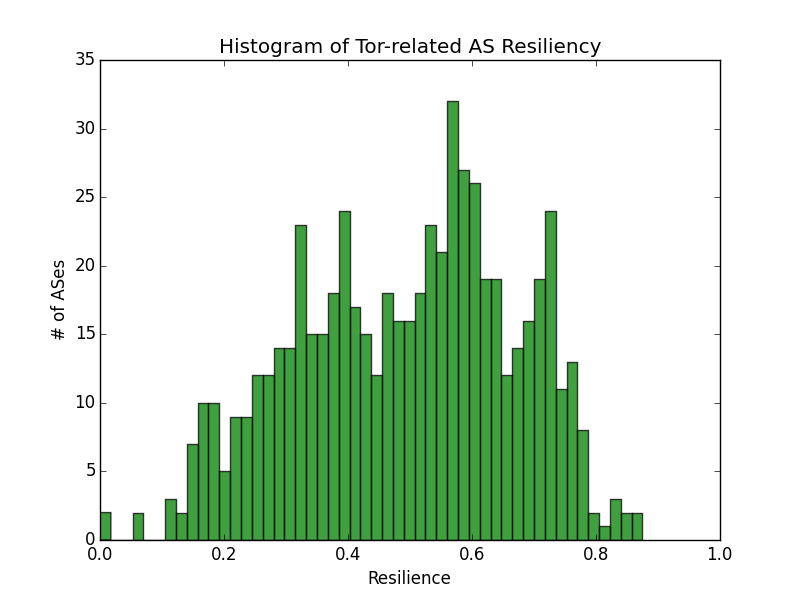
\includegraphics[width=.5\textwidth]{resilience_histogram}
\caption{A histogram of resilience values for all ASes that contain a Tor relay.}
\label{fig:resilience_histogram}
\end{figure}

We then looked at which ASes had the most relays, and what their corresponding resilience is; ideally, ASes with more relays are also more resilient to hijack attacks.  Figure~\ref{fig:res_relays} shows the resilience value for an AS and the AS's corresponding number of relays.  

\begin{figure}
\centering
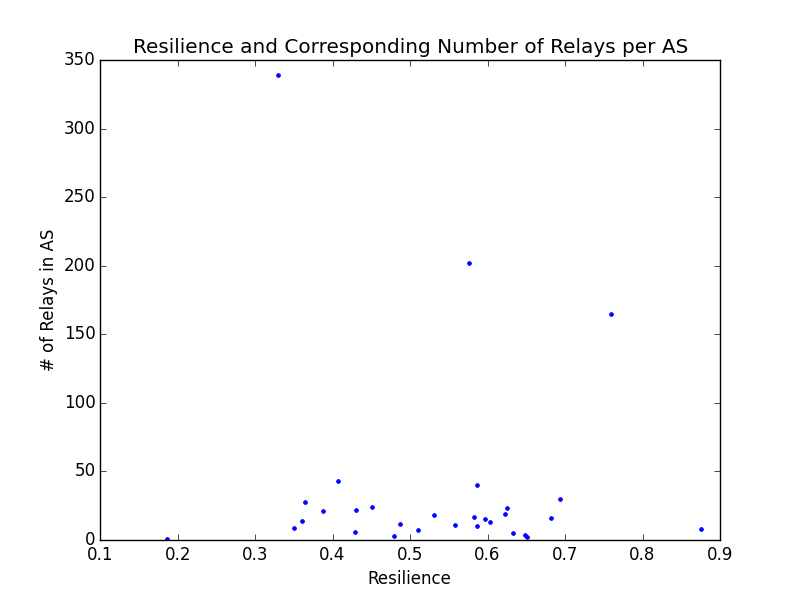
\includegraphics[width=.5\textwidth]{res_num_relays}
\caption{Resilience values for each AS and each AS's corresponding number of relays.}
\label{fig:res_relays}
\end{figure}

We can see one significant outlier - AS16276, OVH - which contains 339 relays; unfortunately, this AS also has a relatively low resilience against hijack attacks.  This motivates our proactive and reactive countermeasures against hijack attacks.

\begin{figure}
\centering
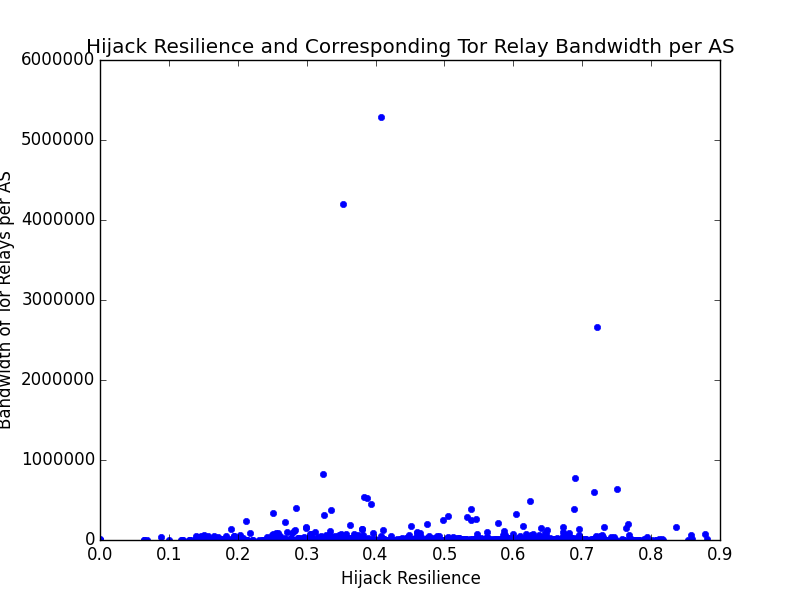
\includegraphics[width=.5\textwidth]{hijack_bandwidth}
\caption{Bandwidth of all Tor relays in an AS, and the corresponding AS hijack resiliency.}
\label{fig:hijack_bw}
\end{figure}

We also conducted our measurements on past data to analyze the hijack resiliency trend on the Tor network.  Figure~\ref{fig:resilience_trend} shows the average AS resiliency to hijack attacks each year.  We can see that the average resiliency has increased since 2008, but still remains below .50.  

\begin{figure}
\centering
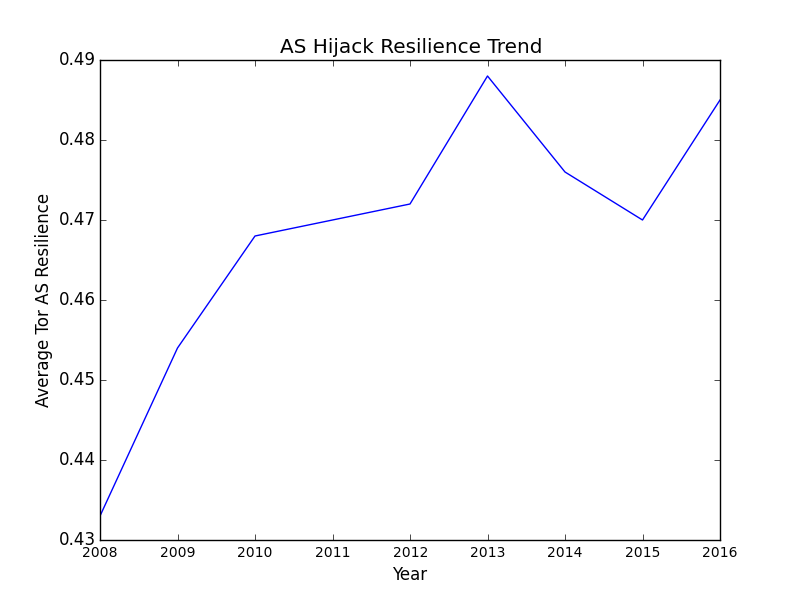
\includegraphics[width=.5\textwidth]{hijack_resilience_trend}
\caption{Average Tor AS resilience each year from 2008-2016.}
\label{fig:resilience_trend}
\end{figure}

\subsection{Interception Resilience Results}

We measured the resilience to interception attacks for each Tor-related AS.  The distribution of interception resilience values is shown in Figure~\ref{fig:interception_histogram}, and we can see that many Tor-related ASes have a much higher resiliency to interception attacks that could be carried out by Tier 1 ASes.  

[More analysis here on interception plots]

\begin{figure}
\centering
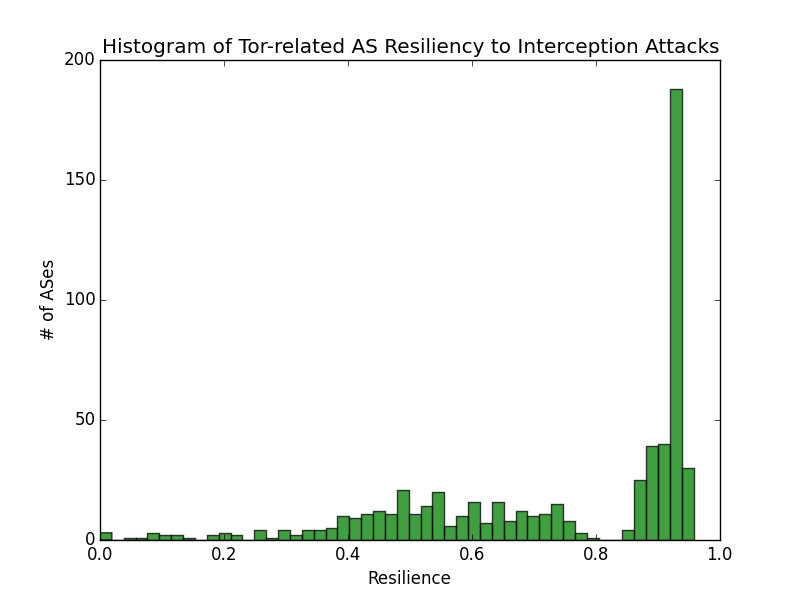
\includegraphics[width=.5\textwidth]{interception_resiliency}
\caption{A histogram of resilience values for all ASes that contain a Tor relay in 2015.}
\label{fig:interception_histogram}
\end{figure}

\begin{figure}
\centering
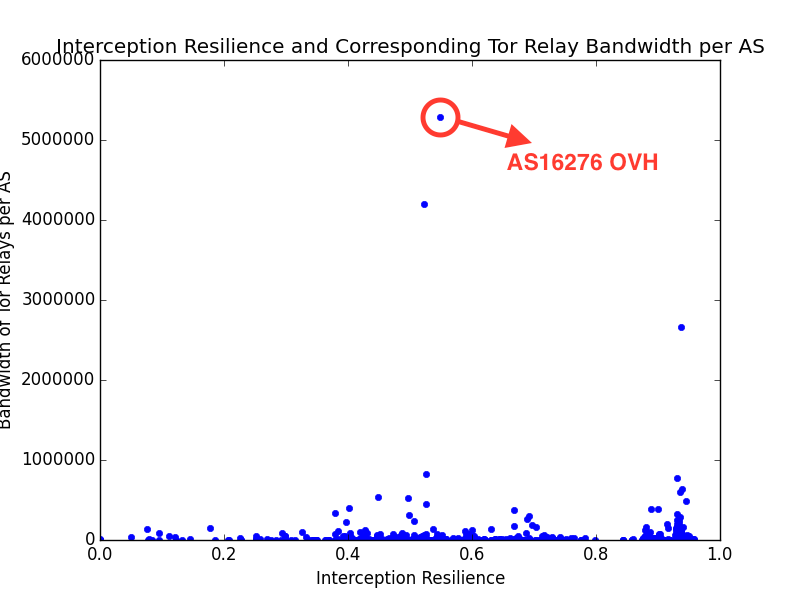
\includegraphics[width=.5\textwidth]{interception_bandwidth}
\caption{Bandwidth of all Tor relays in an AS, and the corresponding AS interception resiliency.}
\label{fig:interception_bw}
\end{figure}

\subsection{Case Study: Indosat 2014}
In 2014, Indosat, one of Indonesia's largest telecommunications networks, announced 417,038 new prefixes, but it usually only announces about 300 prefixes~\cite{indosat2014}.  Previous work found that this compromised 44 Tor relays, 38 of which were guard relays and 17 of which were exit relays (11 hijacked relays were both guards and exits) ~\cite{sun2015raptor}.  We calculated the hijack resilience of the hijacked ASes; the results are shown in Figure~\ref{fig:case_study}.  We can see that the AS hijack resiliency ranges from 0.0 to .76, with most ASes falling in the middle of the spectrum. 
%This means that even ASes with relatively high resilience values (.72 and .76) have the potential to be hijacked.  

\begin{figure}
\centering
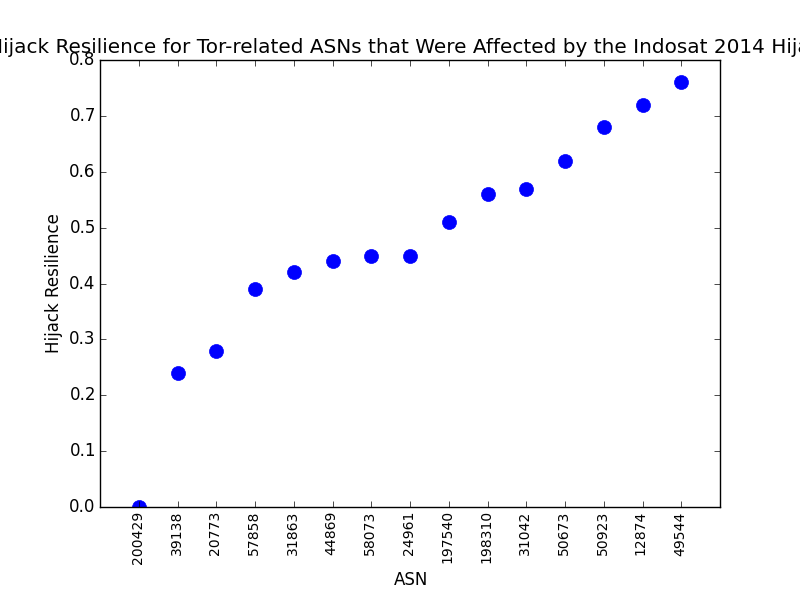
\includegraphics[width=.5\textwidth]{case_study_graph}
\caption{The ASes that contain at least one Tor relay, and were affected by the Indosat hijack attack in 2014, along with their corresponding hijack resiliency values.}
\label{fig:case_study}
\end{figure}
